\documentclass[12pt]{article}
%\usepackage[sf,bf,small,sc]{caption}
\usepackage{graphicx}
\usepackage{color}
\newcommand{\bi}{\begin{itemize}}
\newcommand{\ei}{\end{itemize}}

\title{BreastCal Software Repository}
\author{Arne Vandenbroucke}
\date{\today}
\begin{document}
\sf
\maketitle
\abstract{
This document provides an overview of the analysis software written for the Breast System. The software suite contains many different independent programs as well as a shared library. The software uses many of the ROOT libraries for I/O, data storage and analysis.
}
\newpage
\tableofcontents

\newpage
\section{Software organization}
The software contains many different programs as well as a shared library. 

\subsection{Dependencies}
The software needs ROOT and also the RootMacros.git repository. The latter contains a library with a number of functions that I used in various places, like functions to normalize histograms, perform error propagation, or fitting gaussians for example

\subsection{The {\tt Makefile}}
In order to compile the package you should edit the makefile and specify location of the ROOTMACROS. After that you should do the following steps:
\bi
\item {\tt make .rules}
\item {\tt make}
\ei
The makefile is quite powerfull and will automatically compile all code. It is important to keep the defined extension nomenclature: (1) source code that ends in .cc will be added to the shared library. (2) source code that ends in .C will be compiled at least into objects. (3) source code that starts with a lower case will be compiled into an executable. Some source code only provides functions called by other programs. These need to be labeled starting with an upper case letter and extension .C . 

The dependencies are automatically generated in the {\tt make .rules} step. A combination of `sed' and `awk' processes a `.depend' file into a `.rules' file. This particular code is quite cryptic, but can be easily verified by copying and pasting it onto the command line. It may not be a $100\%$ transferrable to other OS'es. The `.depend' file is generated through compiling with the `-MM' option. 

\subsection{The shared library}
A shared library was implemented so that ROOT would be able to read and understand the classes written to a ROOT file. ROOT handles classes through their names, unlike standard C++, so therefore it needs tis own dictionary. Each class that will be written to a root file needs to be included in the shared library. I also choose to add the Selectors for data analysis to the shared library (see later). The dictionary itself is generated through {\tt rootcint}

\subsection{Design considerations}
The software broadly falls into two phases. A `singles` phase and a `coincidence` phase. The former deals with crystal segmentation, energy calibration and mapping, and needs to be used with any dataset whether data was taken in singles or in coincidence mode. The second phase merges data from the two panels together. Before merging a time sorting step may or may not be needed ( depending on the success of the front-end sorting Aaron Jaffey implemented ) . After merging we will have a `list-mode` file, organized in a Tree, where each line is an event, with a corresponding energy and position in each panel and a time difference. Timing calibration can now be performed, followed by image recon.

Figure~\ref{fig:singlescal} gives an overview of the various programs that are needed to perform calibration. The {\tt calibrate} program provides the acutal calibration, but obviously calibration parameters are needed. These calibration parameters come in the form of a `PixelCal' object, which itself is created by the three programs in the brown boxes. 

\begin{figure}
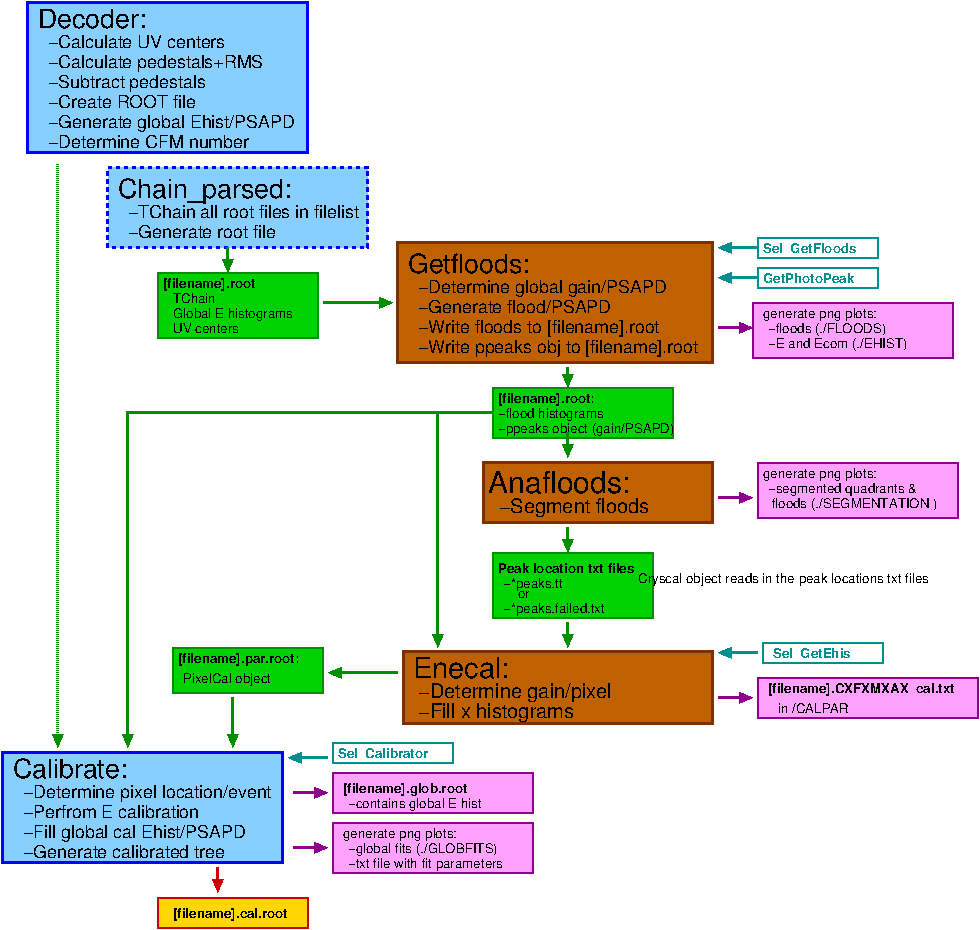
\includegraphics[angle=90,width=.8\textheight]{./SW_Scheme.png}
\caption{schematic of the software}
\label{fig:singlescal}
\end{figure}

\subsection{GIT Branches}
This software project has been an ever evolving endeavor. I started working with a version that was originally in the folder `ANA\_V5'. This version was used up to roughly December 2012. It is very {\tt C}-like and features structs rather than classes. 

Next branch was the `ModuleClass' branch, where some of the structs were replaced by classes for improved I/O. Much of the 2 cartridge data was analysed using this version of the code. Data is organized per chip, module, apd.

Latest branch is the `SpeedUp' branch, where data now is organized per fin rather than per chip. Also, the code uses a more rigorous C++ approach, required by the PROOF mechanism. This lead to the development of a more extended library.

\section{Individual programs Step I}
\subsection{decoder}
The decoder program converts the data generated by each panel into a root tree. It is important to realize that any change in the implementation of the datastream generated by the panels needs to be reflected in this code. The code also is able to calculate pedestals and their RMS; perform pedestal subtraction. The decoder will also generate global uncalibrated energy histograms and assign a cartridge, fin, module and APD number to each event. The program has following input switches:\\
\begin{tabular}{ll}
   -v  &  verbosity switch \\
   -f [] & inputfilename \\
   -o [] & outputfilename \\
   -t [] & threshold for hits \\
   -d  & a debug mode that creates a root ouput file of the first pass \\
   -n  []& no hit threshold in other APD on same module \\
   -pedfile [] & file that contains pedestals\\
   -uv & UV circle centers will be calculated\\
   -uvt []& set uv threshold [ for pulser applications ]\\
   -pos []& in case of point source measurements, the position of the linear stage\\
   -cmap [] & specify which DAQ board nfo file to use rather than the default in \$ANADIR/nfo\\
   -p  & generates .ped file with average and RMS values of the channels \\
   -a  & generate ascii file \\
\end{tabular}
In particular the `-d' option can be quite handy, as it allows a user to look at the data in its most raw form, so you can make sure that the signals look like how they suppose to look like. 

\subsubsection{Limitations} 
Right now the code doesn't handle the channel map. This may be an issue should we be rewiring some output lines to different RENA channels. Doing so may result in `bowtie' floods. Solution would be to read the channel\_map.nfo file. 

\subsection{chain\_parsed}
The DAQ software closes files when a certain filesize is reached (currently 500MB). For a long run you would thus have multiple data files. Chain\_parsed, combines all these files, specified in a `filelist`. This is fairly commonly done in HEP analysis, where many datafiles are chained together in a TChain. For a user a TChain looks like a single TRee. Internally, files will be addressed, so it's important not to move these files, specified in `filelist' to a different location. The output will be a ROOT file that still contains the globale Ehist, and the UV centers\\
\begin{tabular}{ll}
-f []& filelist containing decoded files\\
-o []& optional output filename\\
-v & optional verbosity switch\\
\end{tabular}


\subsection{getfloods}
This program is one of the three programs that actually loops over the entire dataset. It first estimates where the photopeak position is for each APD, using the function {\em GetPhotoPeak}. Once the photopeak is selected, a gated flood histogram is filled. The last step requires data-looping and is done using the PROOF mechanism, which uses multiple processors. PROOF has a load-balancer that distributes work across multiple CPU cores. Whenever PROOF is invocked, I have written Selectors. In this case the selector is called {\em Sel\_GetFloods}. These selectors are a bit tricky as they use the PROOF framework, and as such, their input needs to be read from the `inputlist` to the PROOF process. 

The program will also generate flood histogram plots and global energy histogram plots. The little red triangle in the energy histogram plots are the best estimates for the photopeak. The software adds the flood histograms as well as a {\em ppeaks} object ( containing photopeak position for each APD) to the input root file. \\
\begin{tabular}{ll}
-f []& input file name\\
-v & optional verbosity switch\\
\end{tabular}

\subsection{anafloods}
Program performs segmentation. The program is litterally called {\tt anafloods\_psf\_v2}. It depends on DetCluster, FindNext and Apd\_Sort16. The latter deals with the sequential, heuristic segmentation algortihm, when 16 peaks are identified in each quadrant using TSpectrum::Search. `FindNext' generates the functions used in the pictorial structure program. The program will first try the sequential method. If this sequential method fails, the pictorial structure method is attempted.

The program generates plots of segmented quadrants and plots, and it will output text files with peak location coordinates for each APD. A file with the extension `peaks.failed.txt' is generated is the segmentation failed. It is important to move these files into a directory called {\tt ./CHIPDATA}, because the subsequent program will look for the peaks there. The reason I implemented it like this is twofold: (1) since we have simple text files for each APD, a user can simply edit or even generate these text files should (s)he not be happy with the output of the program. (2) If a user had manually edited the peak location file, and accidentally re-run the anafloods program, these manual edits would be overwritten. To prevent such an accidental overwrite, the user is forced to copy the peak location files to the CHIPDATA folder. 

The program can be recompiled while enabling or disabling some preprocessor definitations to for instance enable or disable pictorial structures, or the generation of several figures. 

The verbosity switch will generate a ton of debug information in case the segmentation failed. I used this info a lot to tune the algorithm. With the -v option enabled, some extra postscript (.ps) files will be generated that will show the algorithm in action. 

Quadrant splitting is done as of May 2014 using a K-means method (k=4).

A user can also specify an individual cartridge, fin, module or apd on which the segmentation would run. This is usefull e.g. for debugging or for module or fin testing where we don't have a full cartridge:\\

\begin{tabular}{ll}
 -f [] & filename\\
 -v & optional verbose\\
 -c []& optional cartridgeId\\
 -l []& optional finId \\
 -m []& optional moduleId\\ 
 -a []& optional apdId\\
 -yoff [] & optional: explicitely specify yoffset for quadrant splitting ( use only if you specify one particular apd with -c X -l Y -m Z -a W )\\
 -xoff [] & optional: explicitely specify xoffset for quadrant splitting ( use only if you specify one particular apd\\
\end{tabular}

\subsection{enecal}
This program will gain calibrate every individual pixel. It requires to loop over the entire dataset again. A histogram for every crystal pixel in the system is generated. As mentioned before, it will read crystal pixel locations from files in the ./CHIPDATA folder. The software will generate a  CXFXMXAX\_cal.txt file in the folder ./CALPAR that includes x,y coordinate of every pixel, as well as the gain and energy resolution for both common and spatial channels. This file is generated through the {\tt pixelcal} object. 

The Sel\_GetEhis class is responsible for looping over the data through PROOF. I have limited the number of nodes to two, as I found that parsing the data together after all parallel sessions are finished takes quite a bit of time. 

The program will also generate histograms of the X-positions, which are added to the inputfile. These are usefull for subsequent FOM analysis. 

The most important outputfile is the `*.par.root' file, which contains all calibration data. That file can then be used by the `calibrate' program to actually perform calibration. After enecal is finished we have calculated all calibration parameters required for singles analysis.

I have experimented with the {\em -map} option so that pixel locations would be stored as histograms which would be read in. As such an easy lookup-table would be used rather than explicitely calculating the distance to each pixel location and finding the minimum distance. These maps are generated with the {\em writefloodmap} program.

\begin{tabular}{ll}
-f []& filename\\
-v & optional verbosity switch\\
-fit & if you only want to do fitting of the Energy histograms (per pixel)\\
-map & see above\\
\end{tabular}

\subsection{calibrate}
This program actually performs calibration. Obviously we need to loop over the data again. If we use PROOF, then events will no longer be time-ordered. So depending on what you want to do, you may want to enable or disable the PROOF mechanism. If the proof mechanism would be disabled, then I would recommend that the program is only run over the decoded input files and not across the entire TChain. This is indicated by the dashed arrow in figure~\ref{fig:singlescal}. A user can launch multiple decoding jobs simultaneously. 

The output of the program is a list-mode datafile organized in a tree. Each event now is organized as a  ModuleCal object. A pixelId is assigned to every event, finetimestamps are calculated and energy responses are calibrated. The workhorse here is the Sel\_Calibrator class. 

The program also performs fitting of the global calibrated energy spectra per APD. This fitting is quite time consuming but allows a quick functionality test of the system, in particular because gain is also determined. All global energy histograms are stored in a {\em *.glob.root} file. The global fit parameters are also written to a text file and plots are generated ( in ./GLOBFITS ) . It should be possible to invoke PROOF to fit the global histograms in parallel but I haven't yet found how to do so. 

Program options are:\\
\begin{tabular}{ll}
-h & print help\\
-c []& use calibration file [] \\
-f []& filename \\
-P & use PROOF\\
-v & verbosity switch\\
-plots & not used\\
\end{tabular}

\subsection{fom\_ana}
This program calculates FOMs and is usefull for performance evaluation. A root file and a text file are created. The input should be the calibrated root file written by {\tt calibrate}. Program options are:
\begin{tabular}{ll}
-f []& filename\\
-v & verbose\\
-c []& cartridgeId\\
\end{tabular}
Because there are many fits involved again, the fom\_ana runs only per cartridge. So you would have to launch the program multiple times in order to calculate fom for all cartridges.

\section{Individual programs Step II}
Step II merges several data streams together. Since coincidence sorting will
be needed it is important that everything remains strictly time ordered. When
performing the merging I have choosen to keep everything memory-resident. As a
consequence files can't be bigger than the physical available memory. In order
to reduce the burden on memory I split the files in different parts {\bf based
  on timestamps}. This is unlike the split performed by the DAQ which is
purely based on size. One noisy trigger could for instance result in many
files for a particular panel, yet the total coarse time would be the same for
all files in the entire dataset. 

One particular shortcoming the repository has ( also in above programs ) is
that the tree name in the file is hardcoded. I am sure there's a better
solution, but for now you need to keep track of how the TTrees are called in
the files. At least an effort should be made to make the TTree names consistent.

\subsection{get\_opt\_split}
This program is very simple. It checks the time needed in between splits so that each file has at most MAXHITS events. We need to run this on each stream (e.g. 2 streams for ethernet, and 8 streams for the USB ), and select the minimum timestep on all these streams. This is done by grepping the output for the {\tt FINDME} keyword. \\

\begin{tabular}{ll}
-h & display help\\
-f []& filename\\
-v & verbose\\
%--L/--R & switch indicating either left or right hand side\\
\end{tabular}

\subsection{merge\_4up}
This code was written to sort the data in each individual four-up board that has 8 RENA chips ( from the USB age) . I guess now it needs to be changed so it works with data from a full cartridge. The code both time sorts and splits the data into multiple {\em parts}. \\

\begin{tabular}{ll}
-f []& filename\\
-v & verbose\\
%-rb []& renaboard\\
-nc []& number of splits\\
-ts []& timeinterval at which to split\\
-lt []& lasttime \\
%--L/--R & switch indicating either left or right hand side\\
\end{tabular}


\subsection{merge\_panel}
This code was written to merge data from multiple 4-up boards together in a
time sorted fashion. {\bf it has a very interesting sorting procedure that I
  may want to use elsewhere}. This program is probably not going to be used
anymore when dealing with etherenet. \\

\begin{tabular}{ll}
-f []&filename\\
-nb [] & number of boards to merge\\
-v & verbose\\
\end{tabular}


\subsection{merge\_coinc}
Performs coincidence sorting. It has an option to perform delayed coincidence sorting, but that only works so-so: in order to estimate randoms through delayed window method, it's better to physically take a delayed coincidence window. From here on the data are stored as instances of the CoincEvent.cc class. This program optionally generates an ascii file as well. The ascii file obviously will be much larger.\\

\begin{tabular}{ll}
-fl [] & `left' file name\\
-fr [] & `right' file name\\
-of [] & outputfilename \\
-d [] & option for delayed window coincidences\\
-a [] & also write an ascii output file\\
-t [] & threshold ( not implemented yet ) \\
-v & verbose\\
\end{tabular}

\subsection{chain\_merged}
Merge the splitted files back together using TChain.\\

\begin{tabular}{ll}
-f [] & filebase\\
-n [] & splits\\
-r & use for randoms \\
-d [] & delayed window for randoms\\ 
-v & verbose\\
\end{tabular}

\subsection{merge\_ana}
Here we're doing some basic analysis. And we optionally also translate crystal, module, fin and cartridge positions into x,y,z coordinates. This code is just an example here if you would want to use ascii code to do FBP in matlab. A more updated code can be found in the {\tt format\_recon} program. You can easily edit this framework to do your own stuff. Right now it selects only photopeak events, and a hard-coded fine time stamp difference. The {\em -r} switch is needed if we're processing randoms, so no cut is activated on the fine time stamp difference. \\

\begin{tabular}{ll}
-f [] & filename \\
-r & select randoms\\ 
-a & generate ascii output\\
-t & threshold ( not implemented yet ) \\
-v & verbose\\
\end{tabular}

\subsection{format\_recon}
This code converts the input into something that Jingyu's recon code can read. Crystal, apd, module, fin and cartridge positions are transformed into x,y,z coordinates. The user needs to specify the panel distance. Currently there are hard cuts on the energy window on this code, but it is straightforward to edit. \\

\begin{tabular}{ll}
-h & display help\\
-v & verbose mode \\ 
-f [] & filename \\
-r & randoms selection \\
-p [] & paneldistance \\
-a & ascii output generated\\
-t [] & fine time window \\
-ft [] & threshold (not yet implemented)\\
-mt [] & maxtime, ignore all entries after this time \\ 
\end{tabular}


\section{Timing calibration}
Timing calibration is performed in discrete steps: there is a program to account for timing offset between APDs, there is code to account for timing offset on each APD, and there is code to correct a possible energy dependence of the timing.

All timing programs add a string to the filename to indicate what exact calibration has been performed. A postscript file with a fit to the energy resolution will also be created. 


\subsection{cal\_apd\_offset}
Code to calibrate apd offset. Dependent on its location in the system, a certain timing offset will be added to each individual APD. This code aims at correcting this offset. Calibration parameters are also written to a text file. As of now some input parameters are exerimental:\\

\begin{tabular}{ll}
-f [] & filename\\
-gf  & use gaussian fit ( instead of calculating the mean )\\
-v & verbose\\
-ft [] & fine time limit for selecting data to perform calibration on\\
$\ldots$ & a couple of experimental parameters exist to select fin, apd or module\\
\end{tabular}

\subsection{cal\_crystal\_offset2}
Calculates offset per individual crystal. There can be differences of up to 20 ns within one array. Calibration factors are written to a text file.  It's called offset2, because I had written some code in the past that uses an average offset for each crystal array, but it didn't work that well. 

Parameters are very similar to the apd offset code:\\

\begin{tabular}{ll}
-f [] & filename\\
-gf  & use gaussian fit ( instead of calculating the mean )\\
-v & verbose\\
-ft [] & fine time limit for selecting data to perform calibration on\\
$\ldots$ & a couple of experimental parameters exist to select fin, apd or module\\
\end{tabular}


\subsection{cal\_edep}
Calculates dependence of timing on energy. It uses profile histograms to estimate the dependencies.


\begin{tabular}{l}
cal\_apd\_offset -f [filename].merged.root\\
cal\_crystal\_offset2 -f [filename].merged.apdoffcal.root\\
cal\_edep -f [filename].merged.apdoffcal.crystaloffcal.root\\
cal\_apd\_offset -f [filename].merged.apdoffcal.crystaloffcal.edepcal.root -ft 30\\
cal\_crystal\_offset2 -f [filename].merged.apdoffcal.crystaloffcal.edepcal.root -ft 30\\
\end{tabular}

\section{Steering scripts and other tools}
\subsection{UTILS directory}
The UTILS directory contains a script to convert the binary list mode LOR file into ascii to the terminal using {\tt hexdump}. It also contains a folder {\tt GENSORT} that calculates the average distance and angles of the line segments in the pictorial structures
\subsection{anascripts}
These scripts can not necessarily be directly used. Often file names and so will be hard-coded. Many of these script were stored from root sessions where I was performing analysis. It's easy to edit and modify them.
\begin{description}
\item[CompareCrystals.sh:] Compares the crystal locations in two different directories, corresponding to two different acquisitions
\item[cryscal.C] Script that generates a 2D map of crystal locations, based on the closest distance to the (8,8) grid of peak locations. The script also plots the voronoi diagram outline ( through difference between bin contents)
\item[doublegaussonstexpo.C:] function that describes a double gaussian, constant and exponent 
\item[fit\_espec.C] Example on how to fit an energy spectrum ( from root\_hist )
\item[fit\_tspec.C] Example on how to fit the timing spectrum with three gaussains and a constant ( from root\_hist )
\item[pattern.C] Used to make the colors of a voronoi histogram
\item[plot\_cartridge\_glob.C] Root macro that plots the energy resolution and gain of each module in a cartridge using a color code. The script uses {\tt plot\_glob.C}
\item[tresfit.C] Example on how to fit the timing spectrum, shows the effect of various calibrations
\item[tspecfit.C] A double gaussian, a constant and a {\it quadratic} exponential. The latter is intended to describe the Compton edge. 

\subsection{bin directory}
\begin{description}
\item[ana\_mc.sh] This was long the working horse for the analysis of the USB based 2 cartridge setup. It features multi-core analysis so that four processors are used
\item[ana\_randoms.sh] Example of how to do delay window coincidences
\item[mod\_ana.sh] Script used to do module analysis with the $2\times 4$ setup.
\item[cleanup.sh] Script that removes some redundant files after analysis.
\item[runall.sh] Older script that runs the decoder
\item[runall\_si.sh] Older script that runs the decoder in `simple' mode (vs PT or LN ).
\item[ana\_v5*] Older versions of ana\_mc.sh
\item[split\_merge.sh] Used to develop splitting and merging

\end{description}

\end{description}

\end{document}

